\subsection{Descripción del problema.}

\vspace*{0.3cm}

Dado un tablero de ajedrez de tamaño $n \times n$ y $k$ caballos que ocupan
inicialmente ciertos casilleros del mismo, el objetivo del problema consiste
en reunir a todos los caballos en un mismo casillero, minimizando la
cantidad total de movimientos realizados. Esta cantidad equivale a la suma
de los movimientos de todos los caballos en el tablero para llegar a dicho
casillero.

Un caballo puede moverse únicamente respetando los movimientos válidos según
las reglas del ajedrez, pero un casillero puede estar ocupado por más de un
caballo simultáneamente.

\vspace*{0.5cm}

\textbf{Ejemplo:}

En un tablero de 8x8, con 3 caballos en las posiciones [2,2], [5,5] y [2,8],
la menor cantidad de saltos posibles es 4, haciendo que los caballos de los
extremos vayan hacia la posición del caballo del medio[5,5], como se puede ver
en la siguiente imagen:

\begin{figure}[htb]
  \begin{center}
      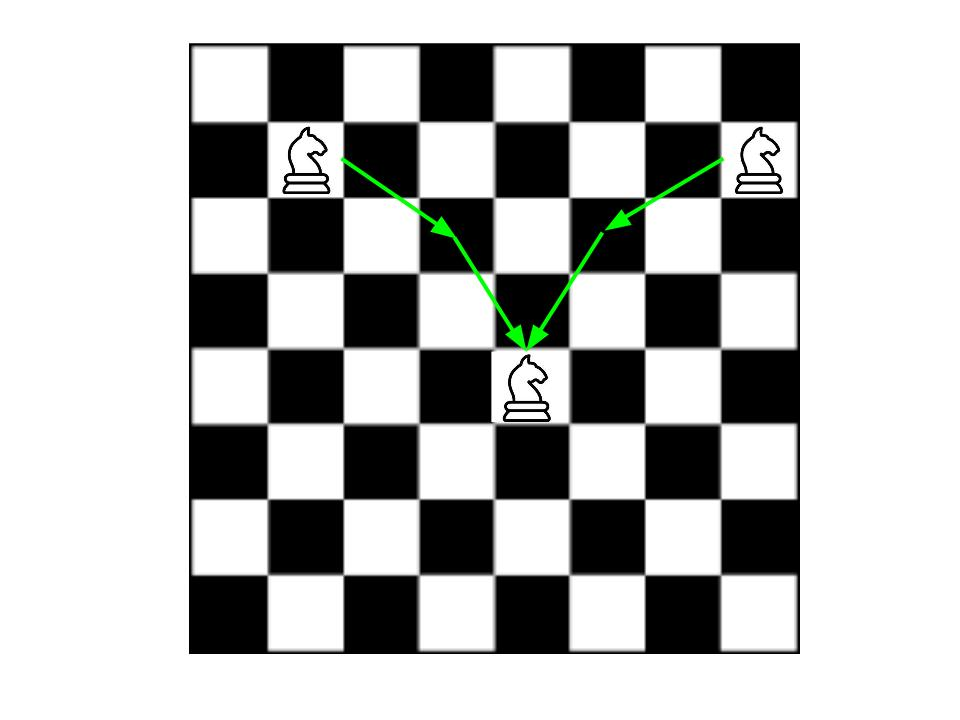
\includegraphics[scale=0.25]{imagenes/caballos.jpg}
  \end{center}
  \caption{ejemplo de tablero.}
\end{figure}



\newpage
\subsection{Desarrollo de la idea y pseudocódigo.}

\vspace*{0.3cm}

Para resolver este problema, utilizaremos $k$ tableros de $n \times n$
casilleros, uno por cada caballo. En cada tablero se calculará el costo para
dicho caballo de llegar a cada casillero, aplicando el algoritmo \textit{BFS} desde el casillero inicial, quedando inválidos los casilleros que no pueden
alcanzarse.

El algoritmo \textit{BFS} consiste en, a partir de un nodo raíz,
recorrer todos los nodos adyacentes a éste (a los que llamaremos vecinos). Estos nodos adyacentes (y la raíz) son agregados a una cola (FIFO) y marcados como visitados. Luego, dado un nodo encolado, si todos sus vecinos fueron visitados, se desencola y se continúa el mismo proceso sobre los nodos restantes (encolando los nodos no visitados cuando encontremos alguno), hasta que esta cola se encuentre vacía, lo cual nos indica que efectivamente hemos alcanzado a todos los nodos del grafo. Sólo se visita una vez cada nodo.

Para poder lograr esto, trataremos al tablero como un grafo (no dirigido), donde los casilleros son los nodos y sus (nodos) vecinos son aquellos casilleros alcanzables desde el nodo de partida, según los movimientos realizables por el caballo. Estos movimientos son las aristas de nuestro grafo.

Luego se recorren todos los casilleros, sumando el valor de estos en todos
los tableros (si son alcanzables), obteniendo así el costo de cada casillero
para cada caballo. De existir, el mínimo de estos valores será el casillero
que pueden alcanzar todos los caballos en la menor cantidad de saltos.

\begin{codebox}
\Procname{$\proc{puntoDeEncuentro}(caballos, n)$}
\li $\id{tableros} \gets \emptyset$
\li \For $caballo \in caballos$ \Do
\li   $\proc{agregar}(tableros,
                      \proc{llenarTablero}(\proc{crearTablero}(n),caballo))$
    \End
\li $\id{i} \gets 0$
\li $\id{j} \gets 0$
\li $\id{min_i} \gets \infty$
\li $\id{min_j} \gets \infty$
\li $\id{min} \gets \infty$
\li \While $\id{i} < \id{n}$ \Do
\li   \While $\id{j} < \id{n}$ \Do
\li     $\id{sum} \gets 0$
\li     \For $tablero \in tableros$ \Do
\li         $\id{sum} \gets \id{sum} + tablero_{ij}$
        \End
\li     \If $sum < min$ \Then
\li       $\id{min} \gets \id{sum}$
\li       $\id{min_i} \gets i$
\li       $\id{min_j} \gets j$
        \End
\li   $\id{j} \gets \id{j} + 1$
      \End
\li $\id{i} \gets \id{i} + 1$
    \End
\li \Return $(\id{min}, \id{min_i}, \id{min_j})$
\end{codebox}


\vspace*{0.3cm}


\begin{codebox}
\Procname{$\proc{crearTablero}(n)$}
\li \Comment $\id{matriz}$ de $n \times n$, inicializada con valores $\infty$
\li \Return matriz
\end{codebox}


\vspace*{0.3cm}


\begin{codebox}
\Procname{$\proc{llenarTablero}(tablero,inicio)$}
\li \Comment Implementación del BFS.
\li \Comment $\id{posiciones}$ es una cola de tuplas $<casillero,costo>$.
\li $\id{posiciones} \gets \emptyset$
\li $\proc{encolar}(posiciones, (inicio,0))$
\li \While $\lnot \proc{vacio?}(posiciones)$ \Do
\li   $\id{pos} \gets \proc{primero}(\proc{frente}(posiciones))$
\li   $\id{nivel} \gets \proc{segundo}(\proc{frente}(posiciones))$
\li   $\proc{desencolar}(posiciones)$
\li   $\id{i} \gets pos_i$
\li   $\id{j} \gets pos_j$
\li   \If $tablero_{ij} \isequal \infty$ \Then
\li     $\id{tablero_{ij}} = nivel$
\li     \For $\id{v} \in \proc{vecinos}(tablero,pos)$ \Do
\li       $\proc{encolar}(posiciones,(v,nivel + 1))$
        \End
      \End
    \End
\end{codebox}



\newpage
\subsection{Justificación de la resolución y demostración de correctitud.}

\vspace*{0.3cm}

La solución es el mínimo número de movimientos entre todos los caballos que
los deja en el mismo casillero, y la posición de ese casillero. Es decir, si
$s \in [1, \dots, n] \times [1, \dots, n]$ es solución, $s$ pertenece a
\begin{align*}
\{p \in [1, \dots, n] \times [1, \dots, n] : \sum_{i = 1}^k
\text{camino\_minimo}(c_i, p) \text{ es mínimo}\}
\end{align*}

Sea $d$ la función de distancia en el tablero, interpretado como grafo del
mismo modo que se menciona en la explicación (ítem 4.2).
Sean $c_1, \dots, c_k \in [1, \dots, n] \times [1, \dots, n]$ las posiciones
iniciales de los $k$ caballos. Definimos $A \in M_{n \times n}(\mathbb{N} \cup
\{+\infty\})$ como $A_{ij} = \sum_{h=1}^k d(c_h, (i, j))$. Si $(p_1, p_2) \in
[1, \dots, n] \times [1, \dots, n]$ es solución, $\sum_{h=1}^k d(c_h, (p_1,
p_2)) = A_{p_1 p_2}$.

Sea $B^h$ la matriz obtenida por el algoritmo al realizar BFS partiendo del
caballo $h$, es decir, $B^h_{ij} = BFS(c_h, (i, j))$. Como BFS calcula el
camino mínimo de un grafo sin peso, se obtiene que $B^h_{ij} = d(c_h, (i, j))$.
Si definimos B como $B_{ij} = \sum_{h=1}^k B^h_{ij}$, entonces, $B = A$, y como
el algoritmo propuesto elige el mínimo $(s_1, s_2)$ en B,
\begin{align*}
  \sum_{h=1}^k d(c_h, (s_1, s_2)) \le \sum_{h=1}^k d(c_h, (p_1, p_2)),
\end{align*}

es decir, $(s_1, s_2)$ es solución.


\newpage
\subsection{Análisis de complejidad.}

\vspace*{0.3cm}

Para el análisis de complejidad nos basaremos en el pseudocódigo de la función
\textsc{puntoDeEncuentro}, correspondiente al ítem \textbf{4.2}.

Se considerará $k$ = cantidad de caballos y $n$ = cantidad de casilleros (los tableros tienen tamaño $n \times n$) y se tendrá en cuenta lo siguiente sobre las estructuras utilizadas en el código y las correspondientes complejidades de sus operaciones:

\begin{itemize}
  \item Todas las operaciones realizadas sobre el contenedor \verb|vector| de la \textit{STL} (size, la creación y manipulación de iteradores) toman tiempo constante $O(1)$. La operación \textit{push_back}, utilizada para agregar elementos al vector, tiene complejidad constante amortizada. La
  operación \verb|resize|, utilizada para definir el tamaño de los vectores, es lineal en el tamaño del contenedor.

  \item Sobre las operaciones realizadas sobre el contenedor \verb|queue| de la \textit{STL}: la cola \textit{posiciones} se crea en tiempo constante. Encolar elementos en \textit{posiciones}, mediante la operación \textit{push}
  toma tiempo constante $O(1)$. Preguntar si una cola es vacía, mediante la operación \textit{empty}, también se realiza en tiempo constante. Acceder al primer elemento de la cola, mediante \textit{front} toma tiempo constante. Desencolar un elemento de \textit{posiciones}, mediante \textit{pop}, también toma tiempo constante $O(1)$.

  \item Los elementos de la cola \textit{posiciones} son \textit{pares} del
  tipo $<Posicion, int>$, donde a su vez, \textit{Posicion}
  es la tupla $<int, int>$. Crear la tupla toma tiempo constante $O(1)$.
  Acceder a la primer ó segunda componente de un par o tupla, mediante
  \textit{first} ó \textit{second}, toma tiempo constante $O(1)$.

\end{itemize}


\textbf{Análisis de complejidad sobre el pseudocódigo de la función principal (puntoDeEncuentro):}

\begin{enumerate}
  \item En la línea 1, creamos el vector vacío \textit{tableros}. Esto se realiza en tiempo constante $O(1)$.

  \item En la línea 2, se realizan $k$ iteraciones (una por cada caballo), por lo que el costo de esta operación es $O(k)$, multiplicado por el costo de
  \verb|agregar| (línea 3). Para determinar el costo de este ciclo for, debemos saber el costo de la operación \verb|agregar| y las funciones que recibe como parámetros (\verb|crearTablero| y \verb|llenarTablero|).

  \item La complejidad de \verb|crearTablero| depende del tamaño del tablero
  (vector de vector). En este caso, creamos un tablero de dimensión
  $n \times n$, por lo cual la complejidad de crearlo es $O(n^2)$. Asignarle valores a cada posición del tablero toma tiempo constante $O(1)$. Luego, la
  complejidad total de la función \verb|crearTablero| es $O(n^2)$.

  \item Analicemos la complejidad de \verb|llenarTablero| (en este ítem, las líneas hacen referencia a esta función y no a la principal). Crear una cola vacía (línea 2) cuesta $O(1)$. Encolar un elemento (línea 3) cuesta $O(1)$. En la línea 4
  tenemos un ciclo que se ejecuta tantas veces como elementos tenga la cola
  \textit{posiciones}. Esta cola contiene como elementos las tuplas
  $<casillero, costo>$, que indican, para cada caballo, el costo (en cantidad de movimientos) que tienen para dirigirse a determinado casillero del
  tablero. En el peor de los casos, en un tablero de dimensión $n \times n$, un caballo puede recorrer todos los casilleros del mismo, por lo tanto su
  cola \textit{posiciones} correspondiente tendría tantos elementos como casilleros a los cuáles moverse, es decir, $n^2$. Por lo tanto, este ciclo
  (línea 4) itera, a lo sumo, $n^2$ veces, teniendo un costo de $O(n^2)$. Veamos el costo de las operaciones que componen este ciclo.
  En las líneas 5 y 6 se realizan 2 asignaciones en $O(1)$, pues se trata de valores enteros. Además, obtener cada componente de la tupla cuesta $O(1)$ y
  acceder al primer elemento de la cola (\verb|frente|) cuesta también $O(1)$.
  \verb|desencolar|, es decir, quitar el primer elemento de \textit{posiciones}, cuesta $O(1)$. Las asignaciones de las líneas 8 y 9 también se realizan en
  tiempo constante por tratarse de valores enteros. En la línea 10, preguntamos si un determinado casillero tiene un cierto valor ($O(1)$) y si
  esto se verifica, realizamos una asignación simple en la línea 11 ($O(1)$) y
  luego, por cada vecino de un determinado casillero (que siempre son 8, por los movimientos permitidos para un caballo), encolamos un elemento en
  $O(1)$. Por lo tanto, la complejidad del ciclo de la línea 12 es $O(1)$, pues la cantidad de operaciones está acotada por una constante
  (cantidad de vecinos) y dentro del ciclo realizamos también operaciones de tiempo constante. Luego, la complejidad de la función \verb|llenarTablero| está acotada superiormente por la complejidad del ciclo de la línea 4, que como vimos anteriormente, es de orden cuadrático. Luego, la complejidad de
  \verb|llenarTablero| es $O(n^2)$.

  \item Por los dos ítems anteriores,
  \verb|llenarTablero(crearTablero(n), caballo)| tiene un costo total de
  $O(n^2) + O(n^2) = 2*O(n^2) = O(n^2)$. Luego, el costo de \verb|agregar| (línea 3 de la función principal) es el costo de agregar (copiar) el tablero de un caballo a \text{tableros}, $O(n^2)$, por lo tanto, el ciclo
  \textit{for} de la línea 2, tiene un costo total de $O(k*n^2)$.

  \item Las asignaciones realizadas (líneas 4-8, 11, 13, 15-19) también se realizan en tiempo constante $O(1)$.

  \item En la línea 12 tenemos un ciclo acotado por la cantidad de elementos de \textit{tableros}, que se corresponde con la cantidad $k$ de caballos, por lo que tiene una complejidad del orden de $O(k)$. La operación realizada dentro es una suma simple que se realiza en tiempo constante.

  \item En las líneas 9 y 10, tenemos un ciclo de, a lo sumo, $n$ iteraciones dentro de otro, también de $n$ iteraciones. Como vimos anteriormente, el ciclo \textit{for} de la línea 12 cuesta $O(k)$, por lo que el ciclo
  \textit{while} de la línea 10 cuesta $O(n*k)$. Po lo tanto, el ciclo más externo, de la línea 9, que contiene a ambos, cuesta $n*O(n*k) = O(n^2*k) = O(k*n^2)$.

  \item Retornar el mínimo entre 3 valores enteros (línea 20) se realiza en tiempo constante $O(1)$.

  \item Por todo lo visto en los ítems anteriores, la complejidad de \verb|puntoDeEncuentro| está determinada por los ciclos de las líneas 2 y 9, ambos del orden de $O(k*n^2)$, pues todas las demás operaciones son del orden      $O(n^2)$, $O(k)$ ó $O(1)$, todas acotadas superiormente por la complejidad
  antes mencionada.

Por lo tanto, la \textbf{complejidad total} del algoritmo implementado para este problema es

\begin{center}
  $O(k*n^2) + O(k*n^2) = 2*O(k*n^2) =$ \textit{\textbf{$O(k*n^2)$}}
\end{center}

\end{enumerate}



\newpage
\subsection{Experimentación y gráficos.}

\vspace*{0.3cm}

\subsubsection{Test 1 - benchmark aleatorio}

(ver \verb|info.2.n.dat|) \medskip

En este test, tenemos $n \times n$ casilleros en cada instancia, con $n$
inicializado en 10 e incrementándose también en 10 hasta alcanzar 1000,
utilizando solamente un caballo.

Para cada instancia se toma el \textbf{valor mínimo} de microsegundos luego de
\textbf{25 corridas}.

\vspace*{0.5cm}

\begin{figure}[h]
  \begin{center}
    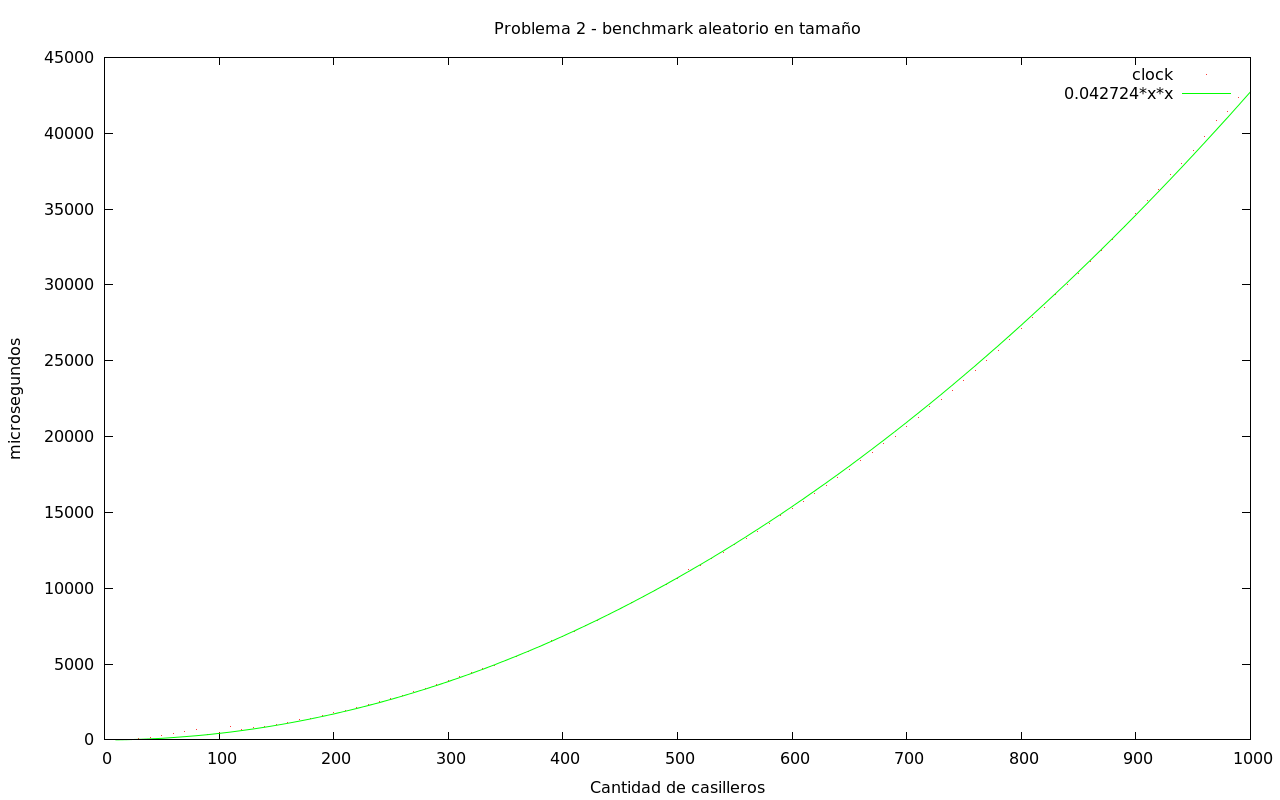
\includegraphics[scale=0.35]{imagenes/grafico-2-n.png}
  \end{center}
\end{figure}

\vspace*{0.5cm}

En este gráfico podemos apreciar que el comportamiento del algoritmo es
claramente cuadrático en la cantidad de casilleros del tablero, tal como se
había estipulado en el análisis teórico de su complejidad. Esto se debe a que,
en este caso, $k$ toma un valor constante (en particular, vale 1), dejando que
la complejidad del algoritmo pase a depender exclusivamente del valor de $n$.


\newpage
\subsubsection{Test 2 - benchmark aleatorio}

(ver \verb|info.2.k.dat|) \medskip

En este test, tenemos un tablero de $500 \times 500$ casilleros en cada
instancia y se varía la cantidad de caballos, comenzando en 10 y aumento este
valor de a 10, hasta alcanzar una cantidad de 1000 caballos.

Para cada instancia se toma el \textbf{valor mínimo} de microsegundos luego de
\textbf{25 corridas}.

\vspace*{0.5cm}

\begin{figure}[h]
  \begin{center}
    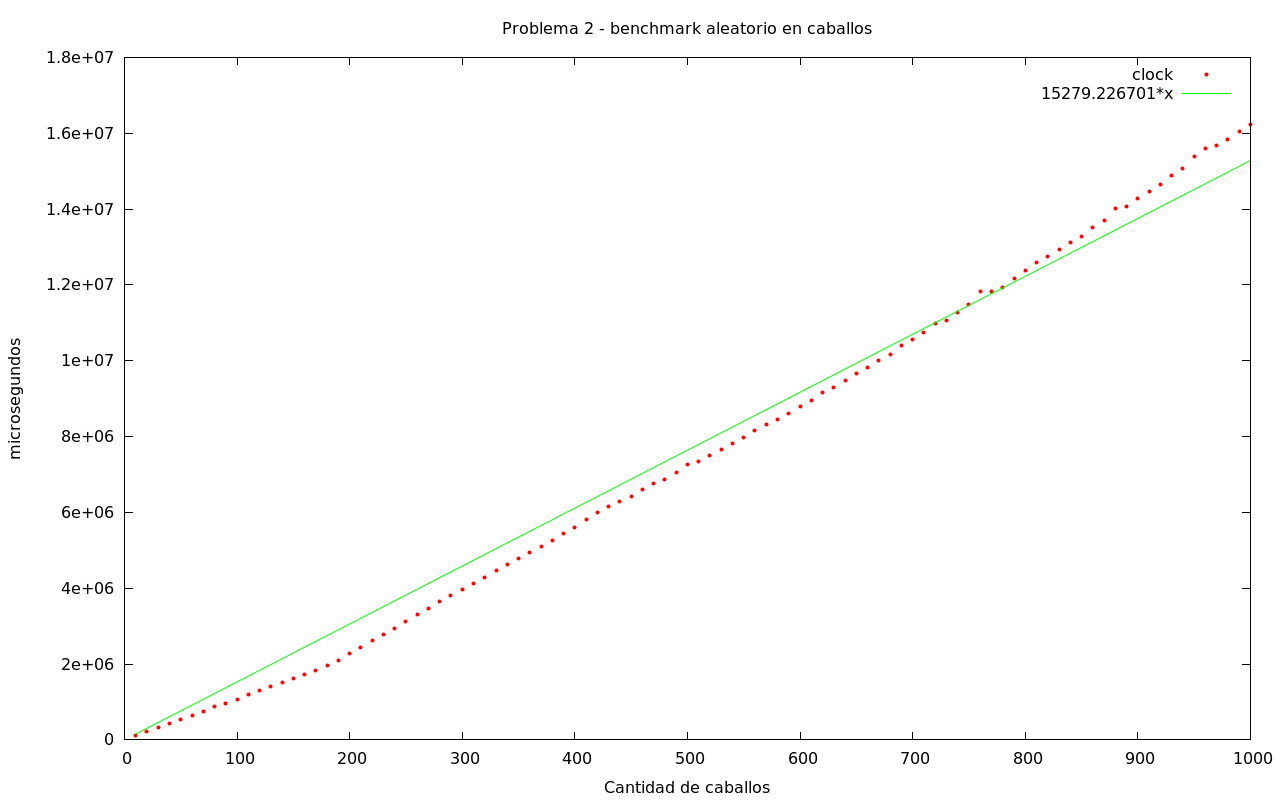
\includegraphics[scale=0.35]{imagenes/grafico-2-k.png}
  \end{center}
\end{figure}

\vspace{0.5cm}

En este gráfico se puede apreciar que el comportamiento del algoritmo tiende a
ser lineal. Creemos que estas pequeñas variaciones pueden deberse a las
optimizaciones realizadas por el compilador y la capacidad del \textit{caché}
de la computadora utilizada para realizar los experimentos. Al empezar con una
pequeña cantidad de caballos, como nuestro algoritmo utiliza una matriz por
caballo, es más sencillo para el procesador distribuir las matrices en las
memorias \textit{caché}, obteniendo así una ganancia en performance al no
tener que ir a buscar a la memoria RAM todas las matrices. Sin embargo, al
aumentar la cantidad de caballos, esto se dificulta cada vez más, dando origen
a las fluctuaciones presentes en el gráfico.
